\newpage
\section{Logistic regression}

Now that we have computed the decision functions for several kernels, we can combine their outputs. Instead of just taking the binary sign of $f(\textbf x)$, we use their continuous values directly.

\subsection{10-dimensional representation}

For each antibody chain $\textbf x$, we build a 10-dimensional vector from the outputs of our 10 SVM kernel tests:
$$
\textbf v(\textbf x) = \bigl(f_1(\textbf x),\, f_2(\textbf x),\, \dots,\, f_{10}(\textbf x)\bigr) \in \mathbb R^{10},
$$
where the components correspond to:
\begin{multicols}{2}
\begin{itemize}
    \item $f_1$: Cauchy
    \item $f_2$: Gaussian (RBF)
    \item $f_3$: Linear
    \item $f_4$: Sigmoid
    \item $f_5$: Tanimoto
    \item $f_6$: Piecewise ($C=0.80$, $W=0.20$)
    \item $f_7$: Piecewise ($C=0.80$, $W=0.08$)
    \item $f_8$: Piecewise ($C=0.82$, $W=0.08$)
    \item $f_9$: Piecewise ($C=0.84$, $W=0.08$)
    \item $f_{10}$: Piecewise ($C=0.78$, $W=0.08$)
\end{itemize}
\end{multicols}

Before training, we standardize every feature using the mean $\mu_k$ and standard deviation $\sigma_k$ measured on the validation set:
$$
\hat f_k(\textbf x) = \frac{f_k(\textbf x) - \mu_k}{\sigma_k}.
$$

\subsection{Model and training}

We take a linear combination of the standardized outputs:
$$
z(\textbf x) = b + \sum_{k=1}^{10} w_k\, \hat f_k(\textbf x),
$$
where $w_k$ is the weight for the $k$-th kernel and $b$ is the bias. The probability of being human is given by the usual logistic function:
$$
P(\text{Human} \mid \textbf x) = \frac{1}{1 + e^{-z(\textbf x)}}.
$$
If $P(\text{Human} \mid \textbf x) \ge 0.5$, we classify the chain as human ($+1$), and murine ($-1$) otherwise.

We train the model on the validation dataset (667 samples) with gradient descent, minimizing the binary cross-entropy loss with an L2 weight penalty:
$$
\mathcal L(\textbf w, b) = -\frac{1}{n}\sum_{i=1}^n \Bigl[y_i \log \hat y_i + (1-y_i)\log(1-\hat y_i)\Bigr] + \frac{\lambda}{2}\sum_{k=1}^{10} w_k^2,
$$
where $y_i \in \{0,1\}$, $\hat y_i = P(\text{Human} \mid \textbf x_i)$, $\lambda = 0.01$, and learning rate $\eta = 0.5$ over 2000 iterations.

\newpage
\subsection{Weights and feature importance}

After training, all learned weights turn out to be positive, meaning that higher scores across all kernels consistently push the prediction towards human. In the following plot, we show the learned weights in descending order:

\begin{figure}[H]
    \centering
    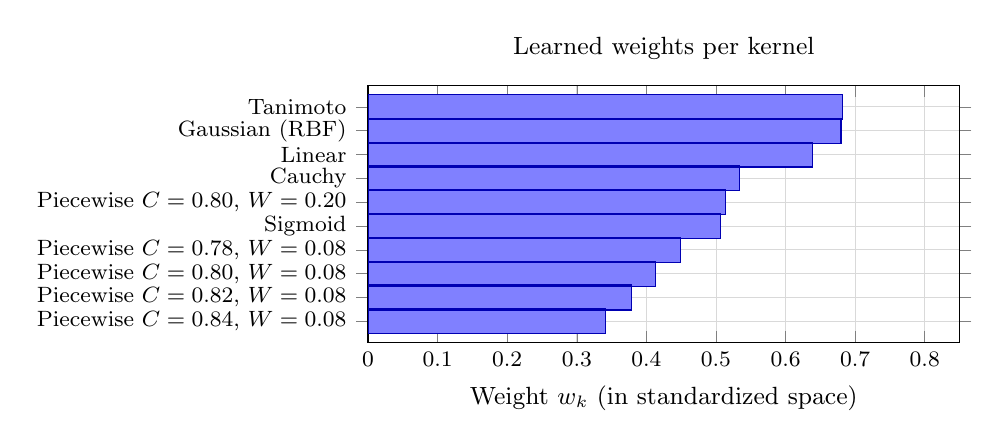
\begin{tikzpicture}
        \begin{axis}[
            xbar,
            width=0.75\textwidth,
            height=0.4\textwidth,
            bar width=9pt,
            xlabel={Weight $w_k$ (in standardized space)},
            ytick={0,1,2,3,4,5,6,7,8,9},
            yticklabels={
                {Piecewise $C=0.84$, $W=0.08$},
                {Piecewise $C=0.82$, $W=0.08$},
                {Piecewise $C=0.80$, $W=0.08$},
                {Piecewise $C=0.78$, $W=0.08$},
                {Sigmoid},
                {Piecewise $C=0.80$, $W=0.20$},
                {Cauchy},
                {Linear},
                {Gaussian (RBF)},
                {Tanimoto}
            },
            xmin=0, xmax=0.85,
            grid=major,
            grid style={line width=0.3pt, draw=gray!30},
            tick label style={font=\footnotesize},
            label style={font=\small},
            title style={font=\small},
            title={Learned weights per kernel},
        ]
            \addplot[fill=blue!50!white, draw=blue!70!black] coordinates {
                (0.3417, 0)
                (0.3789, 1)
                (0.4130, 2)
                (0.4494, 3)
                (0.5070, 4)
                (0.5134, 5)
                (0.5337, 6)
                (0.6382, 7)
                (0.6797, 8)
                (0.6816, 9)
            };
        \end{axis}
    \end{tikzpicture}
    \caption{Learned logistic regression weights in descending order.}
    \label{fig:logreg_weights}
\end{figure}

Tanimoto ($w \approx 0.6816$), Gaussian ($w \approx 0.6797$), and Linear ($w \approx 0.6382$) carry the largest weights, while the narrower piecewise kernels ($W=0.08$) act as fine-tuning corrections right around the decision threshold.

\subsection{Results}

Evaluating the trained model on both datasets gives the following confusion matrices:

\noindent\begin{minipage}{.45\textwidth}\setlength{\parindent}{15pt}
\begin{table}[H]
    \centering
    \renewcommand{\arraystretch}{1.5}
    \begin{tabular}{ccc} \cline{2-3}
        & Human & Murine \\ \hline
    Tagged as human    & 403 & 2 \\ \hline
    Tagged as murine   & 2 & 260 \\ \hline
    \end{tabular}
    \caption*{Validation dataset (667 samples)}
\end{table}
\end{minipage}\hfill\noindent\begin{minipage}{.45\textwidth}\setlength{\parindent}{15pt}
\begin{table}[H]
    \centering
    \renewcommand{\arraystretch}{1.5}
    \begin{tabular}{ccc} \cline{2-3}
        & Human & Murine \\ \hline
    Tagged as human    & 403 & 4 \\ \hline
    Tagged as murine   & 5 & 256 \\ \hline
    \end{tabular}
    \caption*{Test dataset (668 samples)}
\end{table}
\end{minipage}
\vspace{\baselineskip}

On the validation dataset:
\begin{equation*}
    \text{F1}_\text{H} = 0.9951\futnotemath\footnotetext{Precisely: $\text{F1}_\text{H} = 0.995061728395062$.} \qquad
    \text{F1}_\text{M} = 0.9924\futnotemath\footnotetext{Precisely: $\text{F1}_\text{M} = 0.992366412213740$.} \qquad
    \text{Acc} = 0.9940, \quad \mathcal Q = 0.9927
\end{equation*}

And on the test dataset:
\begin{equation*}
    \text{F1}_\text{H} = 0.9890\futnotemath\footnotetext{Precisely: $\text{F1}_\text{H} = 0.988957055214724$.} \qquad
    \text{F1}_\text{M} = 0.9827\futnotemath\footnotetext{Precisely: $\text{F1}_\text{M} = 0.982725527831094$.} \qquad
    \text{Acc} = 0.9865, \quad \mathcal Q = 0.9850
\end{equation*}

\begin{figure}[H]
    \centering
    \begin{tikzpicture}
        \begin{axis}[
            ybar,
            bar width=6pt,
            width=0.75\textwidth,
            height=0.40\textwidth,
            xlabel={Predicted probability $P(\text{Human} \mid \textbf x)$},
            ylabel={Number of sequences},
            xmin=0, xmax=1,
            ymin=0, ymax=380,
            grid=both,
            grid style={line width=0.3pt, draw=gray!30},
            tick label style={font=\small},
            label style={font=\small},
            title style={font=\small},
            title={Distribution of predicted probabilities on the test dataset},
            legend style={at={(0.5,0.92)}, anchor=north,font=\small, draw=none, fill=none},
        ]
            \addplot[fill=blue!60!black, draw=blue!60!black] table[x=bin_mid, y=human_count, col sep=tab] {../results/logreg/test_prob_hist.txt};
            \addlegendentry{True Human}
            
            \addplot[fill=magenta!80!black, draw=magenta!80!black] table[x=bin_mid, y=murine_count, col sep=tab] {../results/logreg/test_prob_hist.txt};
            \addlegendentry{True Murine}
        \end{axis}
    \end{tikzpicture}
    \caption{Distribution of predicted probabilities $P(\text{Human} \mid \textbf x)$ on the test dataset (408 human and 260 murine sequences). Most sequences have probabilities close to 0 or 1, with few sequences near 0.5.}
    \label{fig:logreg_prob_hist}
\end{figure}

\subsection{Permutation importance}

Because our kernels are strongly correlated (as shown in the heatmap), their regression weights are shared and can somewhat mask each kernel's individual contribution. To isolate how much predictive power each kernel brings on its own, we compute the permutation importance on the test dataset: for each kernel, we randomly shuffle its values across the 668 test chains 500 times and measure the resulting drop in accuracy and F1 scores.

\begin{figure}[H]
    \centering
    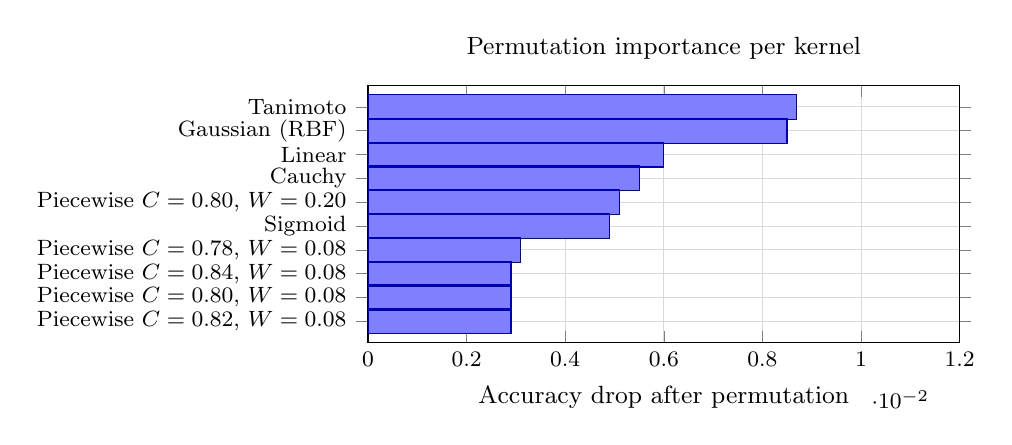
\begin{tikzpicture}
        \begin{axis}[
            xbar,
            width=0.75\textwidth,
            height=0.4\textwidth,
            bar width=9pt,
            xlabel={Accuracy drop after permutation},
            ytick={0,1,2,3,4,5,6,7,8,9},
            yticklabels={
                {Piecewise $C=0.82$, $W=0.08$},
                {Piecewise $C=0.80$, $W=0.08$},
                {Piecewise $C=0.84$, $W=0.08$},
                {Piecewise $C=0.78$, $W=0.08$},
                {Sigmoid},
                {Piecewise $C=0.80$, $W=0.20$},
                {Cauchy},
                {Linear},
                {Gaussian (RBF)},
                {Tanimoto}
            },
            xmin=0, xmax=0.012,
            grid=major,
            grid style={line width=0.3pt, draw=gray!30},
            tick label style={font=\footnotesize},
            label style={font=\small},
            title style={font=\small},
            title={Permutation importance per kernel},
        ]
            \addplot[fill=blue!50!white, draw=blue!70!black] coordinates {
                (0.0029, 0)
                (0.0029, 1)
                (0.0029, 2)
                (0.0031, 3)
                (0.0049, 4)
                (0.0051, 5)
                (0.0055, 6)
                (0.0060, 7)
                (0.0085, 8)
                (0.0087, 9)
            };
        \end{axis}
    \end{tikzpicture}
    \caption{Drop in test accuracy when each kernel is randomly shuffled 500 times. \hyperref[sec:permutation_importance_table]{See appendix for complete table with F1 drops.}}
    \label{fig:permutation_importance}
\end{figure}

Shuffling any of the ten kernels causes a noticeable drop in accuracy, confirming that each one contributes useful information to the final decision. In line with the learned weights, Tanimoto and Gaussian have the largest individual impact.

\subsection{Comparison with decision tree (CART)}

As a baseline comparison, we also trained a decision tree (CART, depth 5) on the exact same 10-dimensional feature vectors. The results on the test set are summarized in Table \ref{tab:logreg_comparison}:

\begin{table}[H]
    \centering
    \renewcommand{\arraystretch}{1.5}
    \begin{tabular}{lcccc} \cline{2-5}
        Model & Accuracy & F1 Human & F1 Murine & $\mathcal Q$ \\ \hline \hline
        CART (depth 5) & $0.9656$ & $0.9714$ & $0.9568$ & $0.9131$ \\ \hline
        Logistic regression & $0.9865$ & $0.9890$ & $0.9827$ & $0.9850$ \\ \hline
    \end{tabular}
    \caption{Test dataset results comparing the decision tree and logistic regression models.}
    \label{tab:logreg_comparison}
\end{table}

The decision tree is held back by its rigid, axis-aligned cuts in the 10-dimensional space, scoring noticeably lower across all metrics ($\mathcal Q = 0.9131$). In contrast, logistic regression combines the continuous margins linearly into a smooth decision boundary, reaching an accuracy of $98.65\%$ and an $\text{F1}_\text{H}$ of $0.9890$.

\subsection{Accuracy and certainty frontier}

To put everything into perspective, we plot the test classification accuracy against our quadratic certainty score $\mathcal Q$ for all individual kernels and the logistic regression model in Figure \ref{fig:model_frontier}:\futnotetext\footnotetext{CART is omitted from the plot since its performance sits well below the axis bounds ($\text{Acc} \approx 0.9656, \mathcal Q \approx 0.9131$).}

\begin{figure}[H]
    \centering
    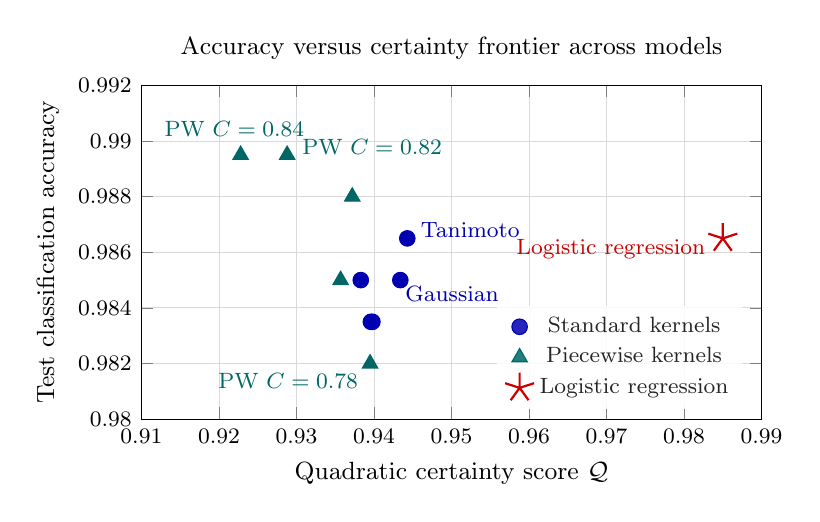
\begin{tikzpicture}
        \begin{axis}[
            width=0.78\textwidth,
            height=0.48\textwidth,
            xlabel={Quadratic certainty score $\mathcal Q$},
            ylabel={Test classification accuracy},
            xmin=0.910, xmax=0.990,
            ymin=0.980, ymax=0.992,
            xtick={0.910, 0.920, 0.930, 0.940, 0.950, 0.960, 0.970, 0.980, 0.990},
            ytick={0.980, 0.982, 0.984, 0.986, 0.988, 0.990, 0.992},
            xticklabel style={/pgf/number format/fixed, /pgf/number format/precision=3},
            yticklabel style={/pgf/number format/fixed, /pgf/number format/precision=3},
            grid=both,
            grid style={line width=0.3pt, draw=gray!30},
            tick label style={font=\footnotesize},
            label style={font=\small},
            title style={font=\small},
            title={Accuracy versus certainty frontier across models},
            legend pos = south east,
            legend style={font=\footnotesize, draw=none, fill=white, fill opacity=0.85},
        ]
            % Standard kernels
            \addplot[only marks, mark=*, mark size=2.8pt, color=blue!70!black] coordinates {
                (0.9383, 0.9850)
                (0.9434, 0.9850)
                (0.9398, 0.9835)
                (0.9396, 0.9835)
                (0.9443, 0.9865)
            };
            \addlegendentry{Standard kernels}

            % Piecewise kernels
            \addplot[only marks, mark=triangle*, mark size=3.2pt, color=teal!80!black] coordinates {
                (0.9372, 0.9880)
                (0.9357, 0.9850)
                (0.9288, 0.9895)
                (0.9228, 0.9895)
                (0.9395, 0.9820)
            };
            \addlegendentry{Piecewise kernels}

            % Meta-classifier
            \addplot[only marks, mark=star, mark size=5.5pt, color=red!80!black, thick] coordinates {
                (0.9850, 0.9865)
            };
            \addlegendentry{Logistic regression}

            % Annotations                                                          0.9850, 0.9865
            \node[anchor=north east, font=\footnotesize, color=red!80!black] at (axis cs:0.9840, 0.9868) {Logistic regression};
            \node[anchor=west, font=\footnotesize, color=blue!70!black] at (axis cs:0.9448, 0.9868) {Tanimoto};
            \node[anchor=west, font=\footnotesize, color=blue!70!black] at (axis cs:0.9428, 0.9845) {Gaussian};
            \node[anchor=south, font=\footnotesize, color=teal!80!black] at (axis cs:0.9220, 0.9898) {PW $C=0.84$};
            \node[anchor=west, font=\footnotesize, color=teal!80!black] at (axis cs:0.9295, 0.9898) {PW $C=0.82$};
            \node[anchor=north east, font=\footnotesize, color=teal!80!black] at (axis cs:0.9392, 0.9820) {PW $C=0.78$};
        \end{axis}
    \end{tikzpicture}
    \caption{Test classification accuracy versus quadratic certainty score $\mathcal Q$ across standard kernels (blue circles), piecewise kernels (teal triangles), and the logistic regression model (red star).}
    \label{fig:model_frontier}
\end{figure}

This frontier highlights the main trade-off: while isolated piecewise kernels achieve slightly higher raw accuracy ($98.95\%$) at the expense of certainty, and standard kernels max out around $\mathcal Q \approx 0.944$, our logistic regression model achieves the best of both worlds. It maintains a high accuracy of $98.65\%$ while dramatically pushing certainty up to $\mathcal Q = 0.9850$, outperforming every single standalone kernel in margin confidence.

